% --------------------------------
% -------  chapter 3  ------------
% --------------------------------
\maketitle
\newpage

\section{Figure or Picture}
  \textbf{Learn how to insert images and caption them. 
    Examples for a single figure, and multiple figures 
    next to each other, using the subfigure environment.}
  \subsection{Captioned images / figures in LaTeX}
    From time to time, it's necessary to add pictures
    to your documents. Using LaTeX all pictures will 
    be indexed automatically and tagged with successive
    numbers when using the \textit{figure environment} 
    and the graphicx package.


    %  lstlisting verbatim minted
    \begin{lstlisting}[language={[LaTeX]TeX}, breaklines=true,frame=single]
      % \begin{verbatim}
        \documentclass{article}
    
        \usepackage{graphicx}
        
        \begin{document}
        
        \begin{figure}
          \includegraphics[width=\linewidth]{boat.jpg}
          \caption{A boat.}
          \label{fig:boat1}
        \end{figure}
        
        Figure \ref{fig:boat1} shows a boat.
        \end{document}
      % \end{verbatim}
    \end{lstlisting}

    \begin{figure}[h!]
      \includegraphics[width=\linewidth]{graphics/boat.png}
      \caption{A boat.}
      \label{fig:boat1}
      \end{figure}
      Figure \ref{fig:boat1} shows a boat. 

    \paragraph{ }
      The figure environment takes care of the numbering and positioning of the image within the document. In order to include a figure, you must use the \textbackslash includegraphics command. It takes the image width as an option in brackets and the path to your image file. As you can see, I put \textbackslash linewidth into the brackets, which means the picture will be scaled to fit the width of the document. As a result smaller pictures are upscaled and larger pictures downscaled respectively. As I mentioned before the brackets contain the path to the image. In this case the image is stored in the same directory as my .tex file, so I simply put boat.jpg here to include it. For large documents, you probably want to store image files in a different folder, say we created a folder images, then we would simply write images/boat.jpg into the braces. In the next command we set a \textbackslash caption, which is the text shown below the image and a \textbackslash label which is invisible, but useful if we want to refer to our figure in our document. You can use the \textbackslash ref command to refer to the figure (marked by label) in your text and it will then be replaced by the correct number. LaTeX is smart enough to retrieve the correct numbers for all your images automatically. Note that you will need to include the graphicx package in order to use this code.




  \subsection{Image positioning / setting the float}

    At some point, you will notice that the figure doesn't 
    necessarily show up in the exact place as you put your 
    code in the .tex file. If your document contains a lot 
    of text, it's possible that LaTeX will put the picture 
    on the next page, or any other page where it finds sufficient 
    space. To prevent this behavior, it's necessary to set 
    the float value for the figure environment.



    \begin{lstlisting}[language={[LaTeX]TeX}, breaklines=true,frame=single]
      %...
      \begin{figure}[h!]
      %...
      \end{lstlisting}

    \paragraph{ }
      The figure environment takes care of the numbering and 
      positioning of the image within the document. In order 
      to include a figure, you must use the \textbackslash includegraphics 
      command. It takes the image width as an option in brackets 
      and the path to your image file. As you can see, I 
      put \textbackslash linewidth into the brackets, which means
      the picture will be scaled to fit the width of the document. 
      As a result smaller pictures are upscaled and larger pictures 
      downscaled respectively. As I mentioned before the brackets 
      contain the path to the image. In this case the image is 
      stored in the same directory as my .tex file, so I simply 
      put boat.jpg here to include it. For large documents, you
      probably want to store image files in a different folder, 
      say we created a folder images, then we would simply write
      images/boat.jpg into the braces. In the next command we 
      set a \textbackslash caption, which is the text shown 
      below the image and a \textbackslash label which is 
      invisible, but useful if we want to refer to our figure 
      in our document. You can use the \textbackslash ref 
      command to refer to the figure (marked by label) in your
      text and it will then be replaced by the correct number. 
      LaTeX is smart enough to retrieve the correct numbers for 
      all your images automatically. Note that you will need to 
      include the graphicx package in order to use this code.

    \paragraph{ }
      Setting the float by adding [h!] behind the figure 
      environment \textbackslash begin tag 
      will force the figure to be shown at the location in 
      the document. Possible values are:
    % list
    \begin{itemize} % list_type 有 enumerate、 itemize 和 description
      \item h (here) - same location
      \item t (top) - top of page
      \item b (bottom) - bottom of page
      \item p (page) - on an extra page
      \item ! (override) - will force the specified location
    \end{itemize} 

    \paragraph{ }
      However, I have only used the [h!] option so far. 
      The float package (\textbackslash usepackage{float}) 
      allows to set the option to [H], which is even stricter than [h!].

  \subsection{Multiple images / subfigures in LaTeX}
      Sometimes when writing a document, adding single images is not optimal, especially when the reader is supposed to compare several results or graphs. In such situations, it might be necessary to use a different environment, called subfigure. The subfigure environment allows you to place multiple images at a certain location next to each other and the usage is pretty straightforward.
    \paragraph{ }
      First you need to add the subcaption package to your preamble:
    \begin{lstlisting}[language={[LaTeX]TeX}, breaklines=true,frame=single]
      \documentclass{article}

      \usepackage{graphicx}
      \usepackage{subcaption}
      
      \begin{document}
      
      %...
      
      \end{document}
    \end{lstlisting}
    \paragraph{ }
      Next, you need to add multiple subfigure environments within a figure environment.
    \begin{lstlisting}[language={[LaTeX]TeX}, breaklines=true,frame=single]
      %...

      \begin{figure}[h!]
        \centering
        \begin{subfigure}[b]{0.4\linewidth}
          
\includegraphics[width=\linewidth]{coffee.jpg}
          \caption{Coffee.}
        \end{subfigure}
        \begin{subfigure}[b]{0.4\linewidth}
          
\includegraphics[width=\linewidth]{coffee.jpg}
          \caption{More coffee.}
        \end{subfigure}
        \caption{The same cup of coffee. Two times.}
        \label{fig:coffee}
      \end{figure}
      
      %...
    \end{lstlisting}
    \paragraph{ }
      Next, you need to add multiple subfigure environments within a figure environment.
    \begin{figure}[h!]
      \centering
      \begin{subfigure}[b]{0.4\linewidth}
        
\includegraphics[width=\linewidth]{graphics/coffee.jpg}
        \caption{Coffee.}
      \end{subfigure}
      \begin{subfigure}[b]{0.4\linewidth}
        
\includegraphics[width=\linewidth]{graphics/coffee.jpg}
        \caption{More coffee.}
      \end{subfigure}
      \caption{The same cup of coffee. Two times.}
      \label{fig:coffee}
    \end{figure}

    \paragraph{ }
    If you look closely, you will see, that I've set the width of the image manually:
    \begin{lstlisting}[language={[LaTeX]TeX}, breaklines=true,frame=single]
      %...
      \begin{subfigure}[b]{0.4\linewidth}
      %...
    \end{lstlisting}

    \paragraph{ }
      and even though there are two images aligned 
      next to each other, their widths are both set
      to 0.4, yet they fill up the whole space. 
      You should always set this value to .1 less
      than you expect. If you want to align three 
      images next to each other, you should 
      consecutively add three subfigures, each
      with a 0.2\textbackslash linewidth. I suggest, if you 
      need some other arrangement, you simply play
      around with the width factor until you 
      are satisfied with the result. A more 
      elaborate example with multiple rows 
      and columns could look like this:
    \begin{lstlisting}[language={[LaTeX]TeX}, breaklines=true,frame=single]
      %...
      \begin{figure}[h!]
        \centering
        \begin{subfigure}[b]{0.2\linewidth}
          
\includegraphics[width=\linewidth]{coffee.jpg}
           \caption{Coffee.}
        \end{subfigure}
        \begin{subfigure}[b]{0.2\linewidth}
          
\includegraphics[width=\linewidth]{coffee.jpg}
          \caption{More coffee.}
        \end{subfigure}
        \begin{subfigure}[b]{0.2\linewidth}
          
\includegraphics[width=\linewidth]{coffee.jpg}
          \caption{Tasty coffee.}
        \end{subfigure}
        \begin{subfigure}[b]{0.5\linewidth}
          
\includegraphics[width=\linewidth]{coffee.jpg}
          \caption{Too much coffee.}
        \end{subfigure}
        \caption{The same cup of coffee. Multiple times.}
        \label{fig:coffee3}
      \end{figure}
      %...
    \end{lstlisting}


    \paragraph{ }
      This will print out the following figure in your document:
      \begin{figure}[h!]
        \centering
        \begin{subfigure}[b]{0.2\linewidth}
          
\includegraphics[width=\linewidth]{graphics/coffee.jpg}
           \caption{Coffee.}
        \end{subfigure}
        \begin{subfigure}[b]{0.2\linewidth}
          
\includegraphics[width=\linewidth]{graphics/coffee.jpg}
          \caption{More coffee.}
        \end{subfigure}
        \begin{subfigure}[b]{0.2\linewidth}
          
\includegraphics[width=\linewidth]{graphics/coffee.jpg}
          \caption{Tasty coffee.}
        \end{subfigure}
        \begin{subfigure}[b]{0.5\linewidth}
          
\includegraphics[width=\linewidth]{graphics/coffee.jpg}
          \caption{Too much coffee.}
        \end{subfigure}
        \caption{The same cup of coffee. Multiple times.}
        \label{fig:coffee3}
      \end{figure}

    \paragraph{Summary}
      \begin{itemize} % list_type 有 enumerate、 itemize 和 description
        \item Use the graphicx package and figure environment to embed pictures
        \item Pictures will be numbered automatically
      \item Change the width of your image by using \begin{verbatim} \includegraphics[width=\linewidth]{} \end{verbatim}
        \item Refer to pictures in your document by setting a \textbackslash label and using the \textbackslash ref tag
        \item Set the position of your image by adding a float option such as [h!]
        \item If you want to show multiple figures next to each other, use the subcaption package and the subfigure environment
      \end{itemize} 
